\documentclass{article}
\usepackage{geometry}
\usepackage{ctex}
\usepackage{graphicx}
\usepackage{float}
\geometry{a4paper, scale=0.8}

\title{计算机系统结构Cache替换策略设计实验}
\author{ZhaohengLi 201750025\\cainetatum@foxmail.com\\15801206130}

\begin{document}
\maketitle

\section{实验背景}
在终端设备上随着游戏的画质、特效、帧率需求的日渐增长,使得这些场景下的访存密集型特点越发显著,对内存的带宽需求不断增长,最终造成游戏场景下芯片功耗的大幅增加。现有处理器主要采用 Cache-Memory层次存储结构,通过Cache缓存频繁访问的程序和数据,减少对内存的访问。然而目前在游戏场景下,SoC芯片System Cache的命中率非常低,需要重新优化Cache替换策略,提高Cache的命中率。

\section{实验目的}
深入理解Cache结构设计及Cache替换策略的原理,阅读Cache替换策略方面的最新研究进展,设计自己的Cache替换策略,提高游戏场景下的Cache命中率。

\section{主流替换策略设计思想}

\subsection{Random替换策略}
随机替换策略不考虑Cache存储的情况,简单地根据一个随机数选择一块替换出去。

随机替换策略在硬件上容易实现,速度非常快,缺点则是命中率方面表现较差。

\subsection{FIFO替换策略}
FIFO(First in First out)算法核心思想为先进先出,即如果一个数据最先进入缓存中,则应该最早淘汰掉。也就是说,当缓存满的时候,应当把最先进入缓存的数据给淘汰掉。

这种替换策略实现简单,操作快速,但是在命中率方便表现一般。

\subsection{LRU替换策略}
LRU(Least Recently Used)算法是把CPU近期最少使用的块替换出去。这种替换方法需要随时记录Cache中各块的使用情况,以便确定哪个块是近期最少使用的块。每块设置一个计数器,Cache每命中一次,命中块计数器清零,其他各块计数器增1。当需要替换时,将计数值最大的块换出。

这种替换策略在命中率方面表现很好,但是在每一次访问Cache时需要较大的计算量,时间复杂度较高。

\subsection{LFU替换策略}
LFU(Least Frequently Used)算法将一段时间内被访问次数最少的那个块替换出去。每块设置一个计数器,从0开始计数,每访问一次,被访块的计数器就增1。当需要替换时,将计数值最小的块换出,同时将所有块的计数器都清零。

这种替换策略将计数周期限定在对这些特定块两次替换之间的间隔时间内,不能严格反映近期访问情况,新调入的块很容易被替换出去。

\subsection{RRIP替换策略}
RRIP(Re-Reference Interval prediction)算法核心思想为将访问间隔较小的块留在Cache中,从而提高命中率。维护Mbits记录PPRV,选择PPRV值为2的M次方减一的项替换出去,如果没有该项,则每项PPRV值+1,之后重复扫描。新进块PPRV置为2的m次方-2,命中块清零。采用此种方法描述访问间隔并通过访问间隔来预测访问概率。

这种替换策略在命中率方面表现很好,缺点则是每一次访问Cache时需要较大的计算量,时间复杂度较高。

\subsection{Clock替换策略}
Clock算法具体的实现方式为定义环形页表,指针指向初始位置,当命中时,将对应页表中的访问位定义为真。当缺失时,从指针位置开始进行判断,如果当前位置访问位为真,将访问位置为假,指针指向下一位,直到指针指向位置的访问位为假,则当前位置为要进行替换的位置,并将指针指向下一位。

这种替换策略综合考虑了FIFO替换策略和LRU替换策略,先进先出替换策略完全不考虑过去的做法,而LRU考虑的时间较长,时钟替换策略既考虑过去,考虑的时间又不是那么长。时钟替换策略的思路是对页面的访问情况进行大致统计。

\section{设计替换策略}
\subsection{替换策略核心思想}
访问Cache的目的是为了缩短获取数据的时间,这就意味着所有的替换策略都需要在提高命中率与减少访问计算量之间进行衡量取舍。

我设计的Swing替换策略如下:

\begin{figure}[H]
    \centering
    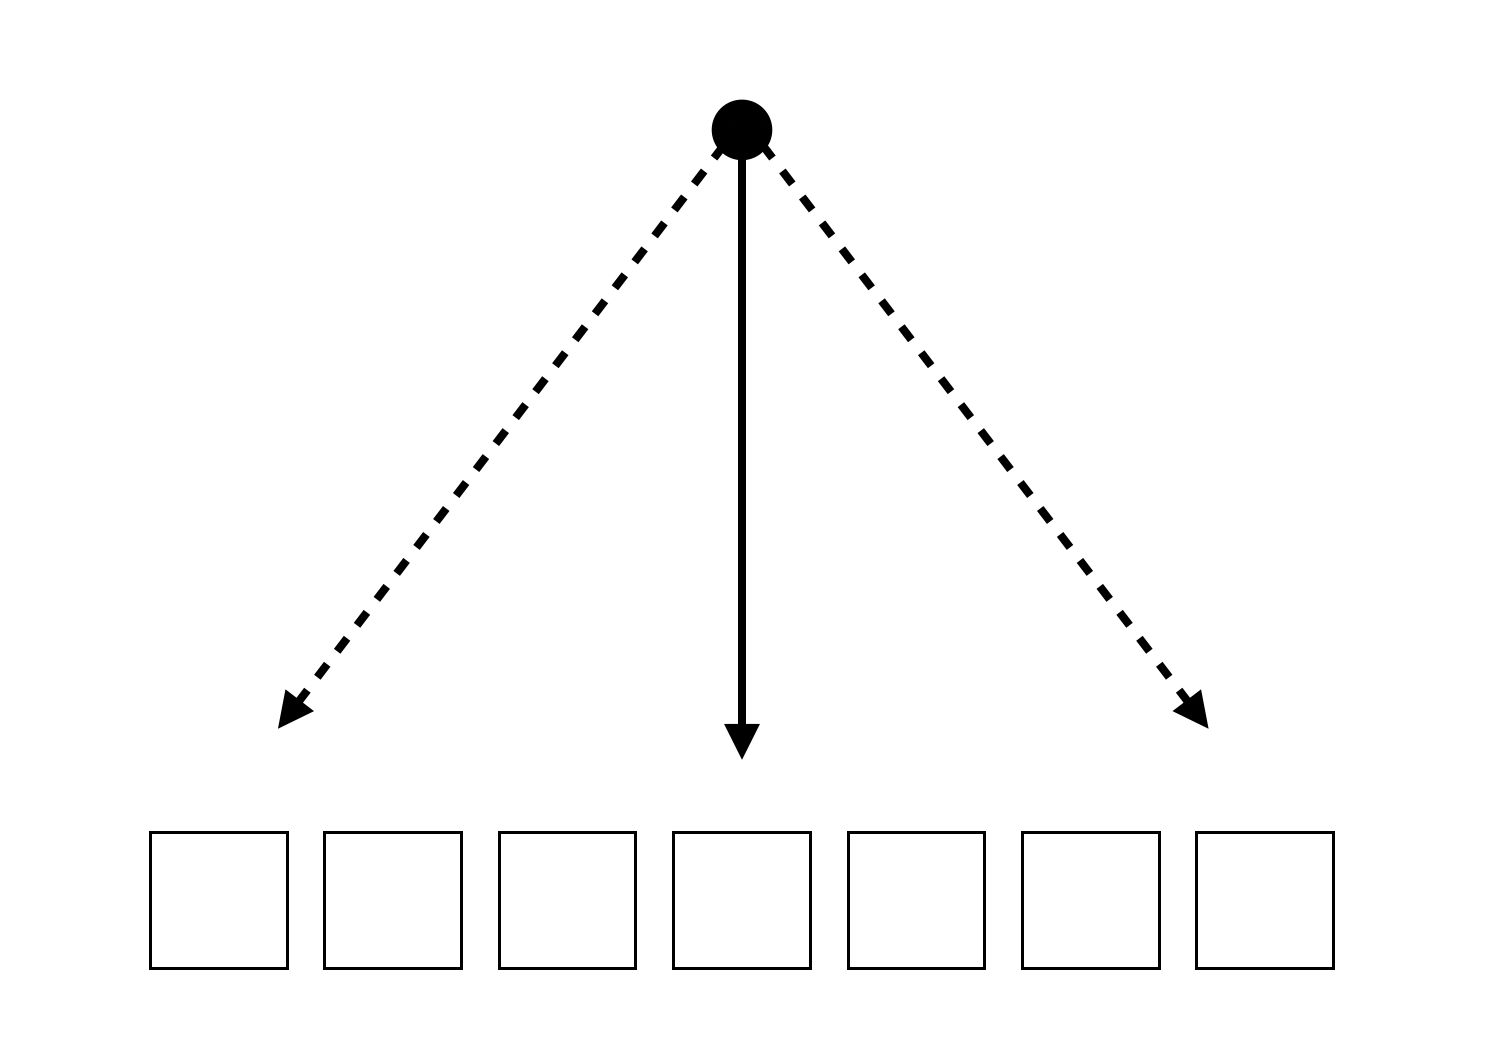
\includegraphics[width=0.7\textwidth]{pic1.png}
    \caption{Swing替换策略示意图}
\end{figure}

图中的矩形代表着Cache块,Cache块上方为“淘汰摆”,其像重力摆一样做简谐运动,“淘汰摆”当前所指向的位置是下一个待替换的Cache块,当访问Cache未命中时,“淘汰摆”所指向的Cache块被替换,同时“淘汰摆”指向下一个Cache块。

当Cache初始化时,“淘汰摆”指向Index为0的Cache块,向此Cache块装入内容后,“淘汰摆”指向Index为1的Cache块,类似地不断进行下去。

假设Cache共有n个,当“淘汰摆”指向Index为n的Cache块时,向此Cache块装入内容后,“淘汰摆”指向Index为n-1的Cache块,由此之后,“淘汰摆”向相反方向摆动。

类似地,当“淘汰摆”再次指向Index为0的Cache块时,向此Cache块装入内容后,“淘汰摆”指向Index为1的Cache块,像重力摆一样做简谐运动。

由于在每次访问Cache的时候没有任何额外计算量,该替换策略可以保持极快的访问速度。命中率方面的表现将在下一小节进行具体分析。


\begin{itemize}
\item{\textbf{时间复杂度$O(1)$}(每次访问Cache时无额外计算量。)}
\item{\textbf{空间复杂度$O(N)$}($N$为Cache组相连路数,用于记录“淘汰摆”指向的位置。)}
\end{itemize}

\subsection{适用场景分析以及命中率分析}
在一般的文件系统中,对文件的访问方式有以下几种:
\begin{itemize}
\item{\textbf{顺序访问:}ABCDEFGHIJKLMNO...}
\item{\textbf{循环访问:}ABCDEABCDEABCDE...}
\item{\textbf{聚簇访问:}ABCDEDCBABCDEDC...}
\item{\textbf{概率访问与随机访问}}
\end{itemize}
对于顺序访问、概率访问、随机访问这三种形式,Cache替换策略的设计对综合访问速度的影响不大,因此Cache替换策略设计的越简单越好,以减少每次访问时的计算量。另外,对这些情况来说,增加Cache的容量是提升综合访问速度较为有效的方法。

接下来对Swing替换策略在循环访问、聚簇访问和随机访问三种访问方式进行命中率分析:

\subsubsection{循环访问方式测试}

Swing替换策略时间复杂度与FIFO替换策略的时间复杂度相同,再此将Swing替换策略和FIFO替换策略进行比较。

下面进行循环访问序列的理论分析。

不难发现,当循环序列长度小于Cache块个数时,所有替换策略均可以保证在循环序列加载完毕后的访问一直命中,因此不分析这种情况。

我们假设Cache块共有4个,循环序列长度为5。模拟的访问过程如下图所示,为了节省空间,最初的装填过程未在图中表示出,从Cache装满开始的访问过程如下图表格所表示。

\begin{figure}[H]
    \centering
    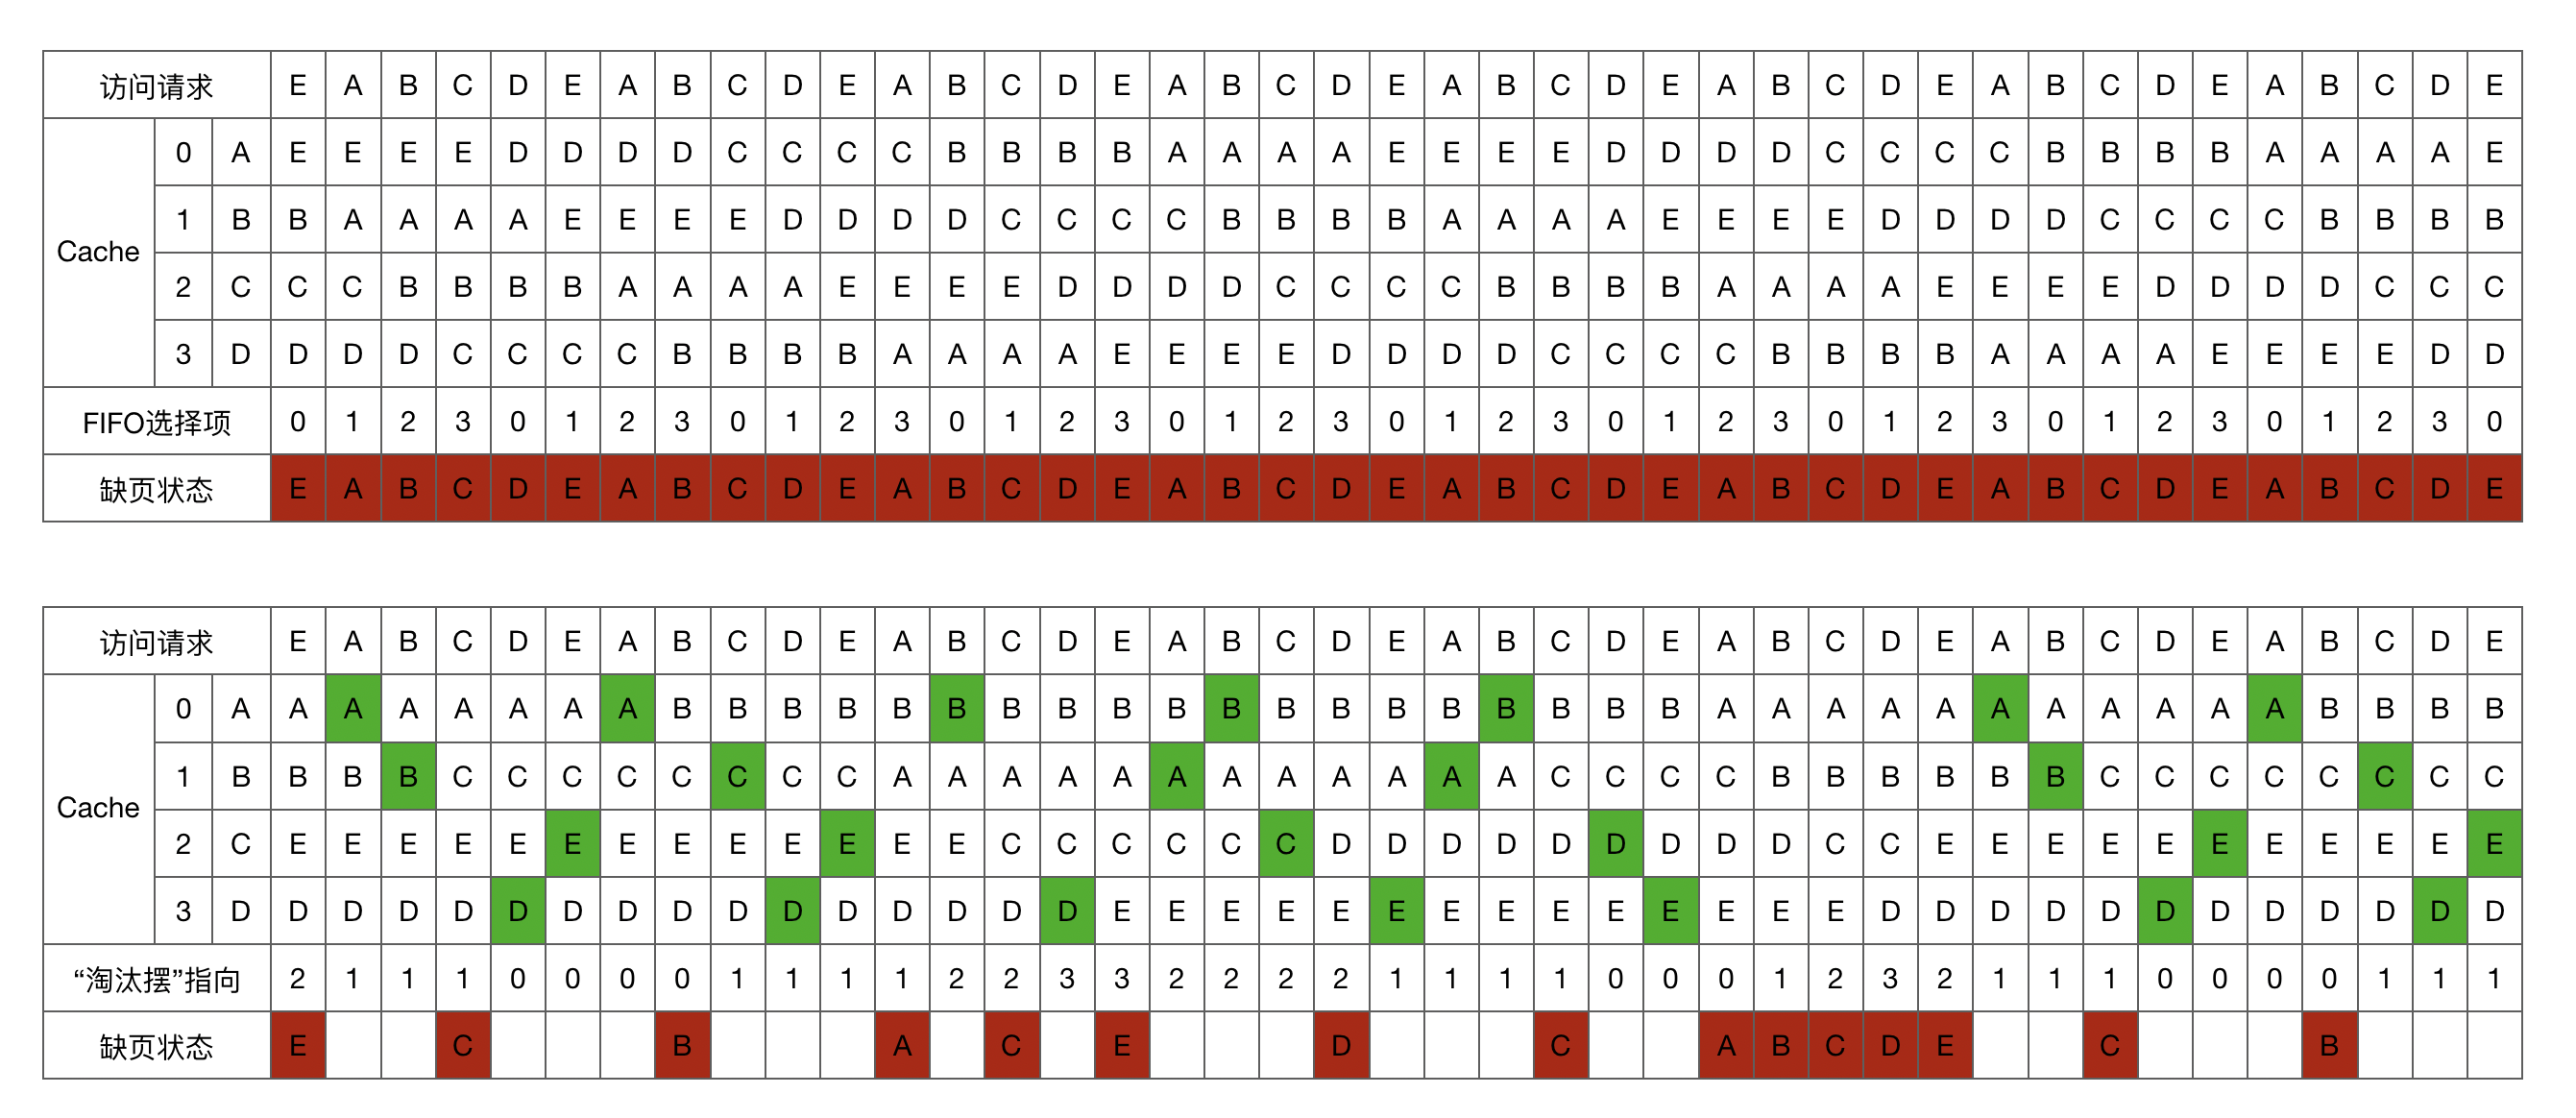
\includegraphics[width=1\textwidth]{pic2.png}
    \caption{FIFO替换策略(上)和Swing替换策略(下)在访问循环序列的表现}
\end{figure}

可以发现,FIFO在进行循环序列的访问时有一个致命缺陷。当循环序列的长度大于Cache块的长度时,会导致访问Cache一直不命中。然而在Swing替换策略中,这个缺陷被修复了,而且在访问循环序列的过程中保持着很高的命中率$(63.4146\%)$。同时可以发现,使用Swing替换策略访问循环序列时,访问过程是也是有循环规律的,这就保证了命中率不会有大幅波动,在不断循环中命中率会趋向一个稳定的数值。

设Cache块个数为$n$,循环序列长度$m$,需要注意的是,当$m>1.5n$时,Swing所表现出来的优势也消失了。

\subsubsection{聚簇访问方式测试}

同样使用Swing替换策略与FIFO替换策略进行比较。不难发现,当聚簇序列长度小于Cache块个数时,所有替换策略均可以保证在循环序列加载完毕后的访问一直命中,因此不分析这种情况。

我们假设Cache块共有4个,聚簇序列长度为5。模拟的访问过程如下图所示,为了节省空间,最初的装填过程未在图中表示出,从Cache装满开始的访问过程如下图表格所表示。

\begin{figure}[H]
    \centering
    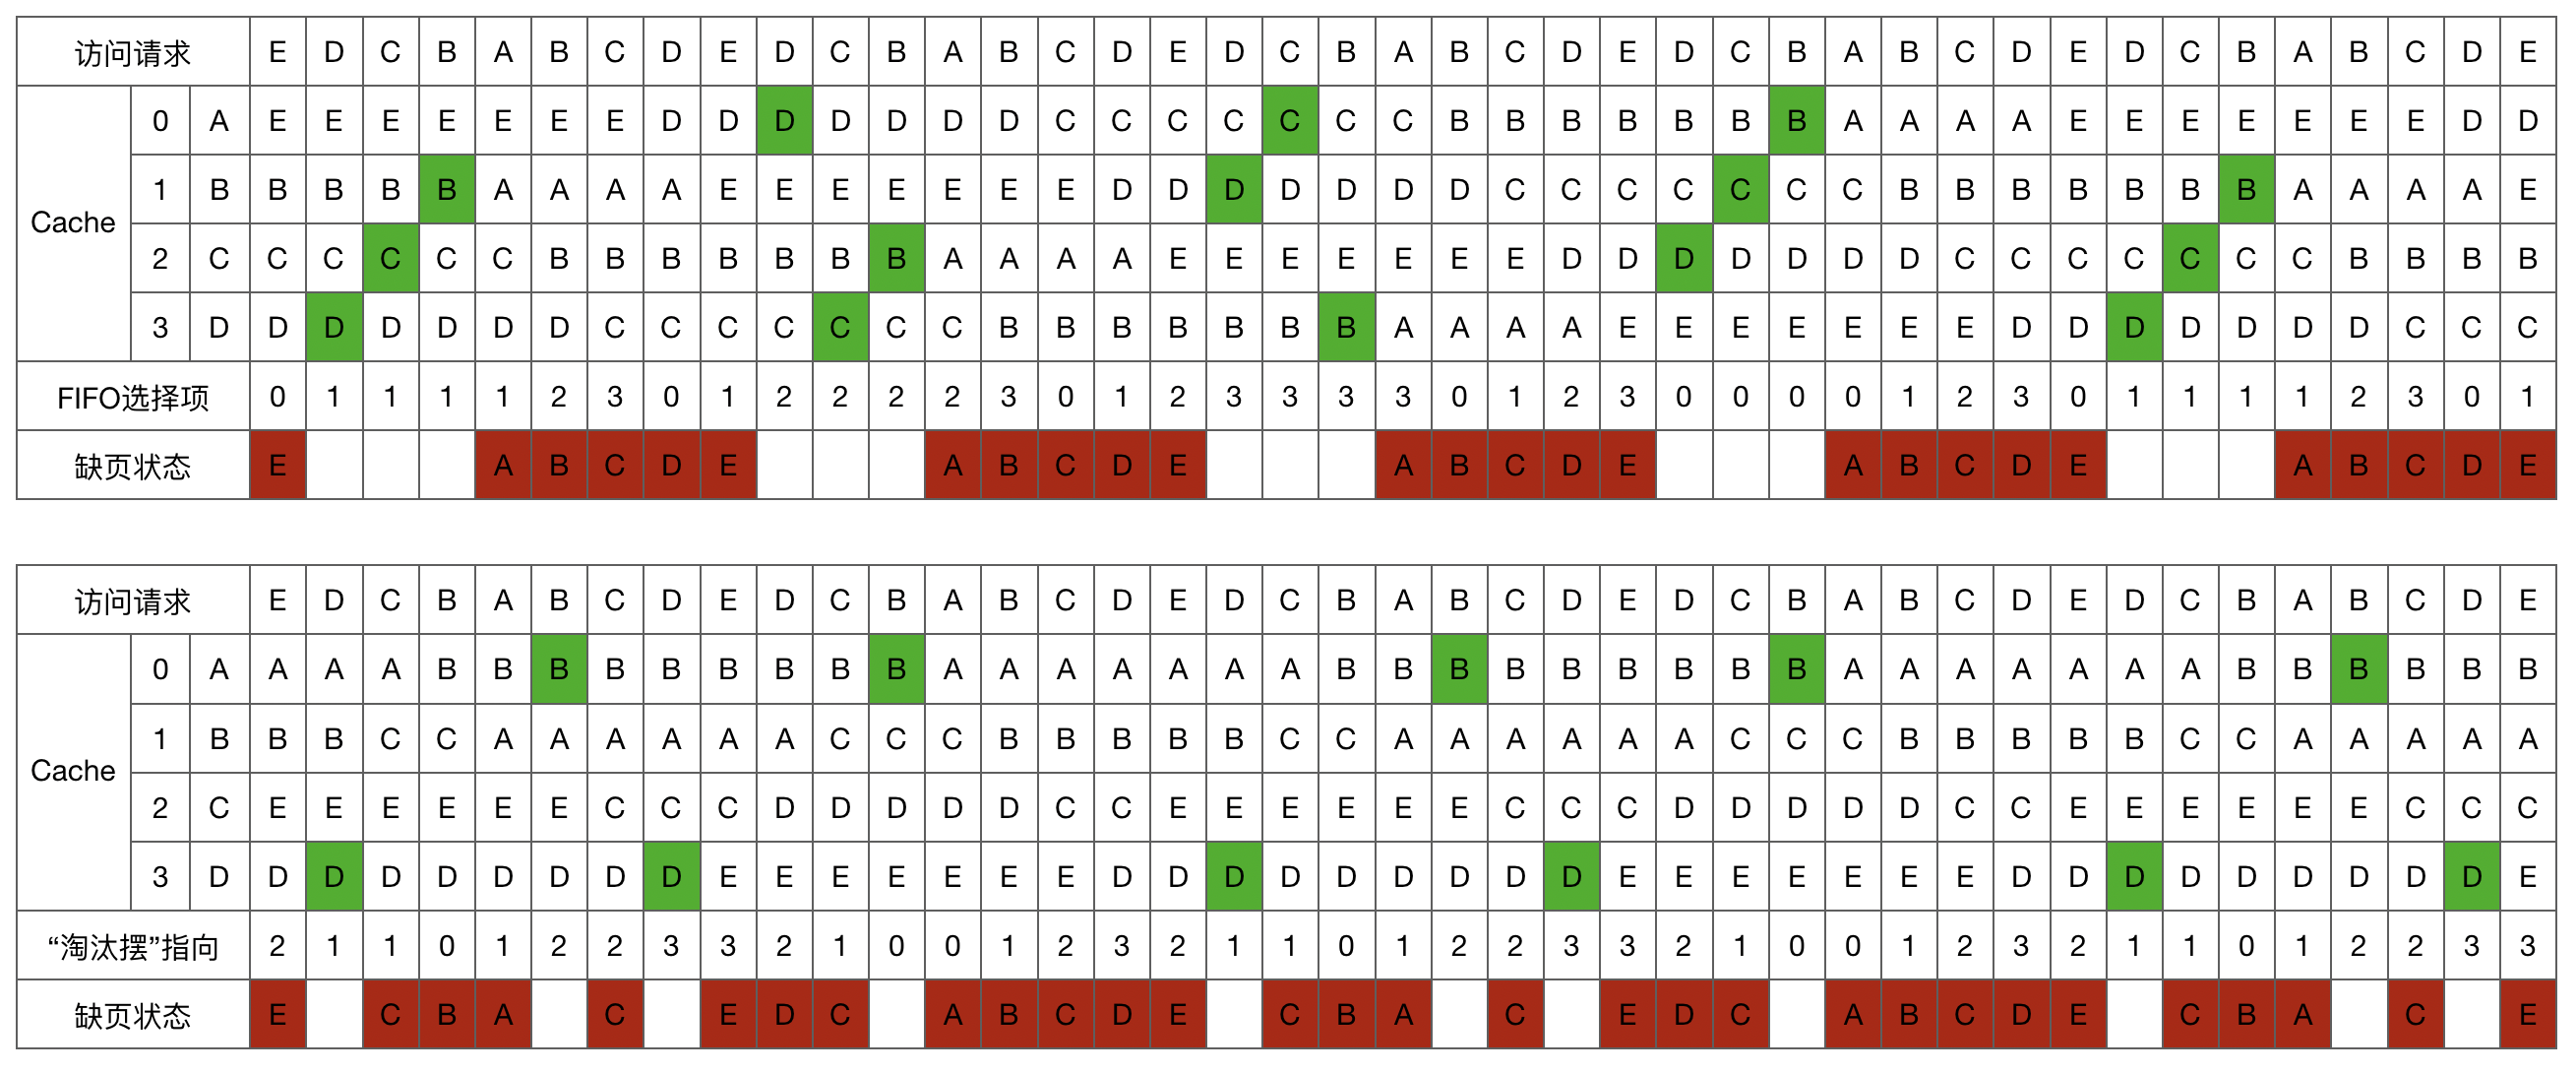
\includegraphics[width=1\textwidth]{pic3.png}
    \caption{FIFO替换策略(上)和Swing替换策略(下)在访问聚簇序列的表现}
\end{figure}

可以发现,FIFO替换策略在进行聚簇序列的访问时要好于Swing替换策略,这是因为FIFO替换出的是最先进入Cache的块,这序列的特点十分吻合,因此取得了不错的命中率$(36.5854\%)$。

Swing替换策略的命中率略低,为$(26.8293\%)$,这是由于在“淘汰摆”摆动到两端的时候,经常会把刚刚进入的Cache块再次替换出去,导致Swing替换策略与聚簇序列的特点发生冲突,通过增大Cache块的数量可以有效缓解这一现象。

可以发现,Swing替换策略在访问聚簇序列的时候,访问过程有循环规律,这就保证命中率不会大幅波动,在不断循环中命中率会趋向一个稳定的数值。

\subsubsection{随机访问方式测试}

我们假设Cache块共有4个,从操作系统课程的案例中取一段随机访问序列,随机序列中有6个可能出现的数值。模拟的访问过程如下图所示,为了节省空间,最初的装填过程未在图中表示出,从Cache装满开始的访问过程如下图表格所表示。

\begin{figure}[H]
    \centering
    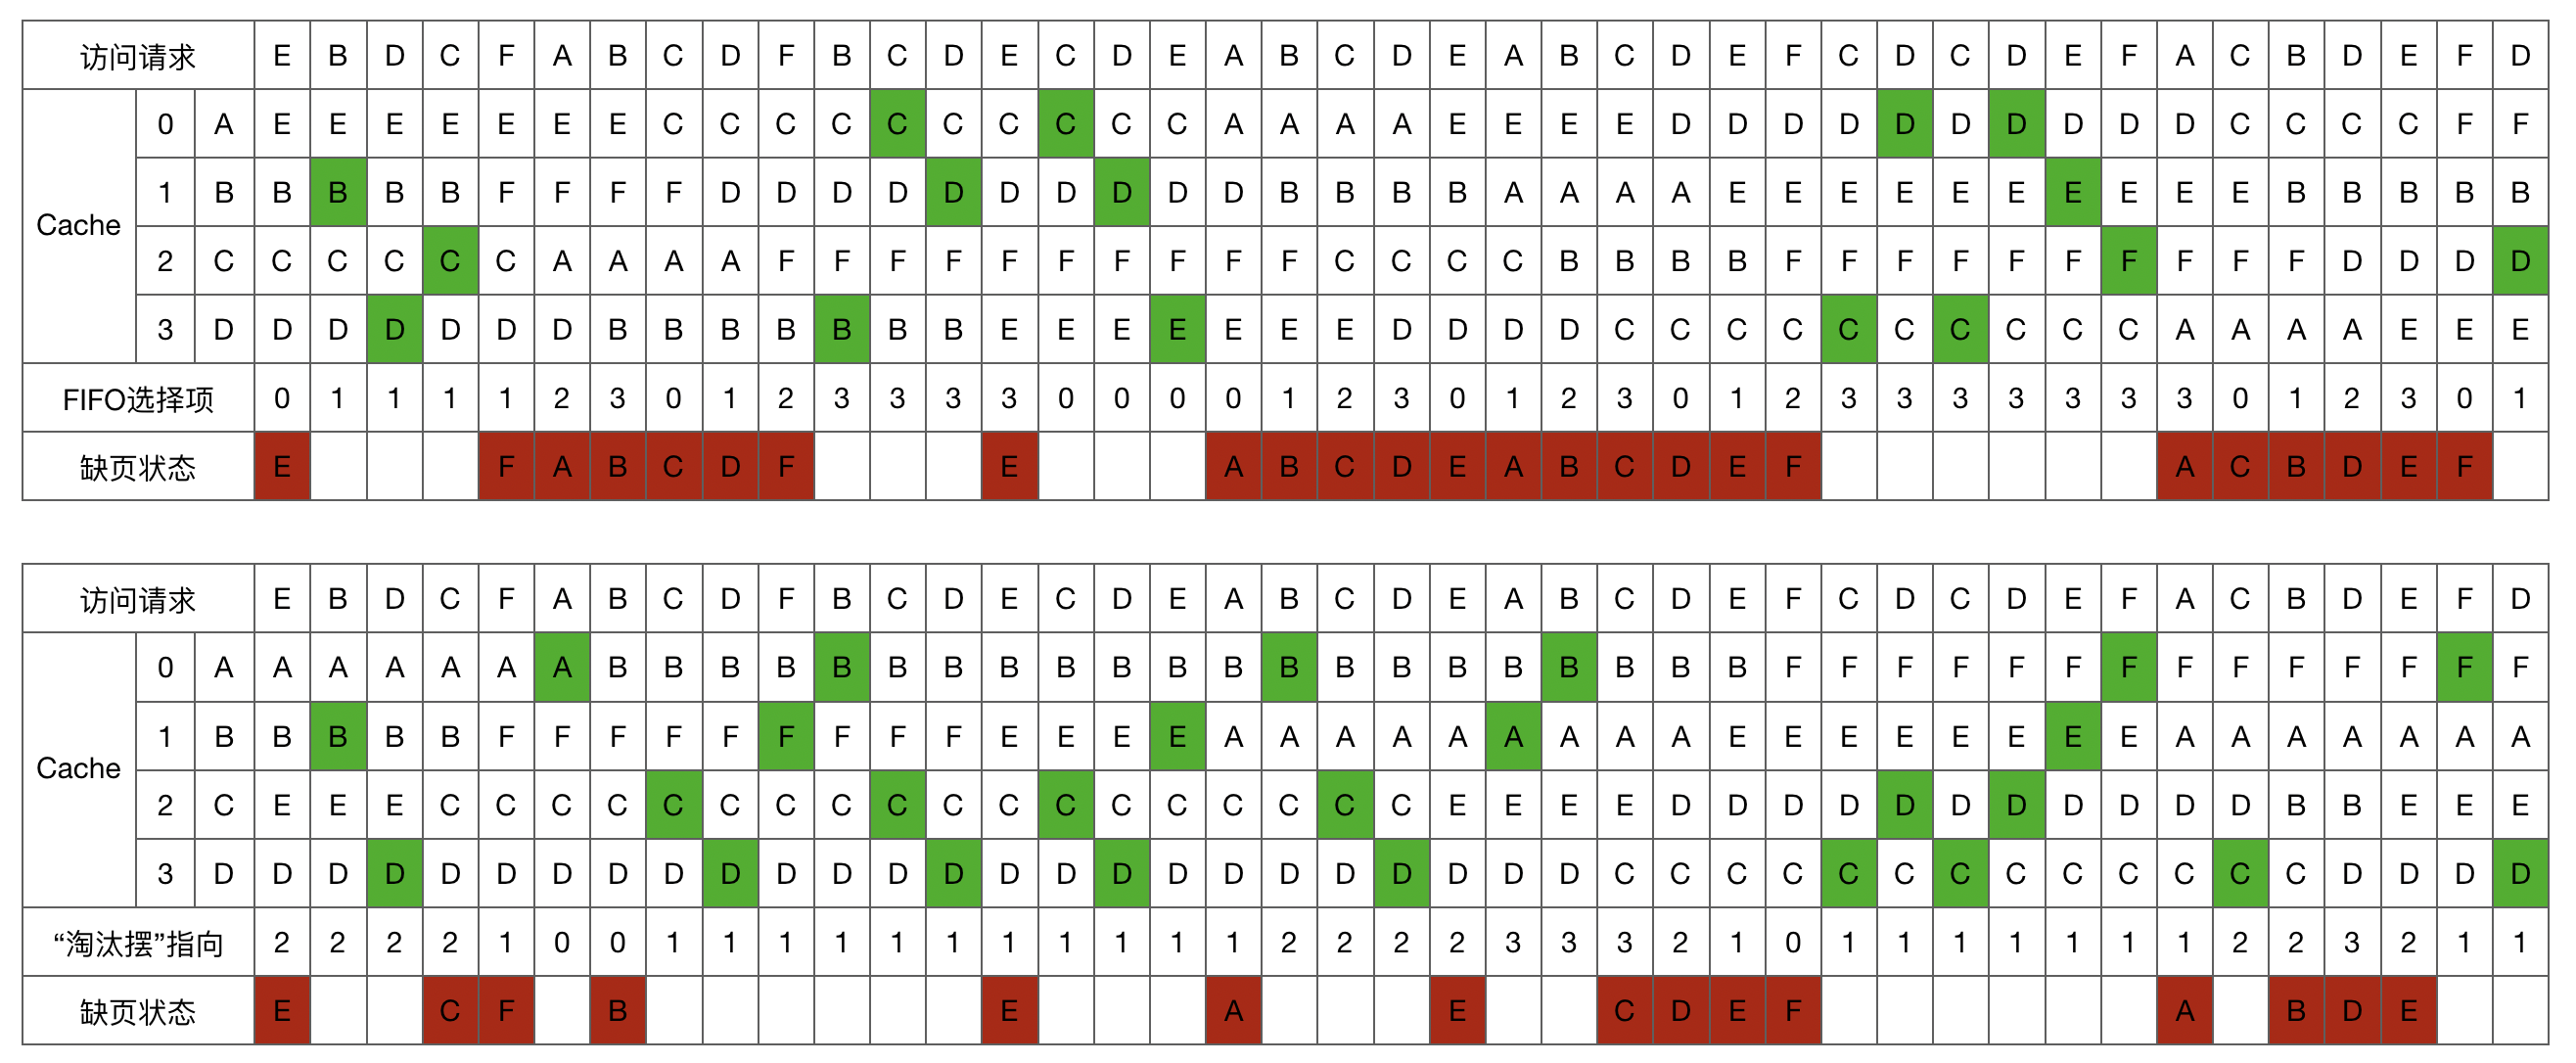
\includegraphics[width=1\textwidth]{pic4.png}
    \caption{FIFO替换策略(上)和Swing替换策略(下)在访问随机序列的表现}
\end{figure}

可见Swing替换策略的命中率$(63.4146\%)$高于FIFO替换策略的命中率$(39.0244\%)$。

\subsubsection{Swing替换策略优势分析}
\begin{itemize}
	\item{Swing替换策略时间复杂度为$O(1)$。}
	\item{Swing替换策略可以很好的应对循环序列访问。}
	\item{Swing的“淘汰摆”在摆动到Cache块队列端点时有“长短时自适应”性质。}
\end{itemize}
长短时自适应性质:

当“淘汰摆”即将摆动到Cache块队列端点时,如图所示。
\begin{figure}[H]
    \centering
    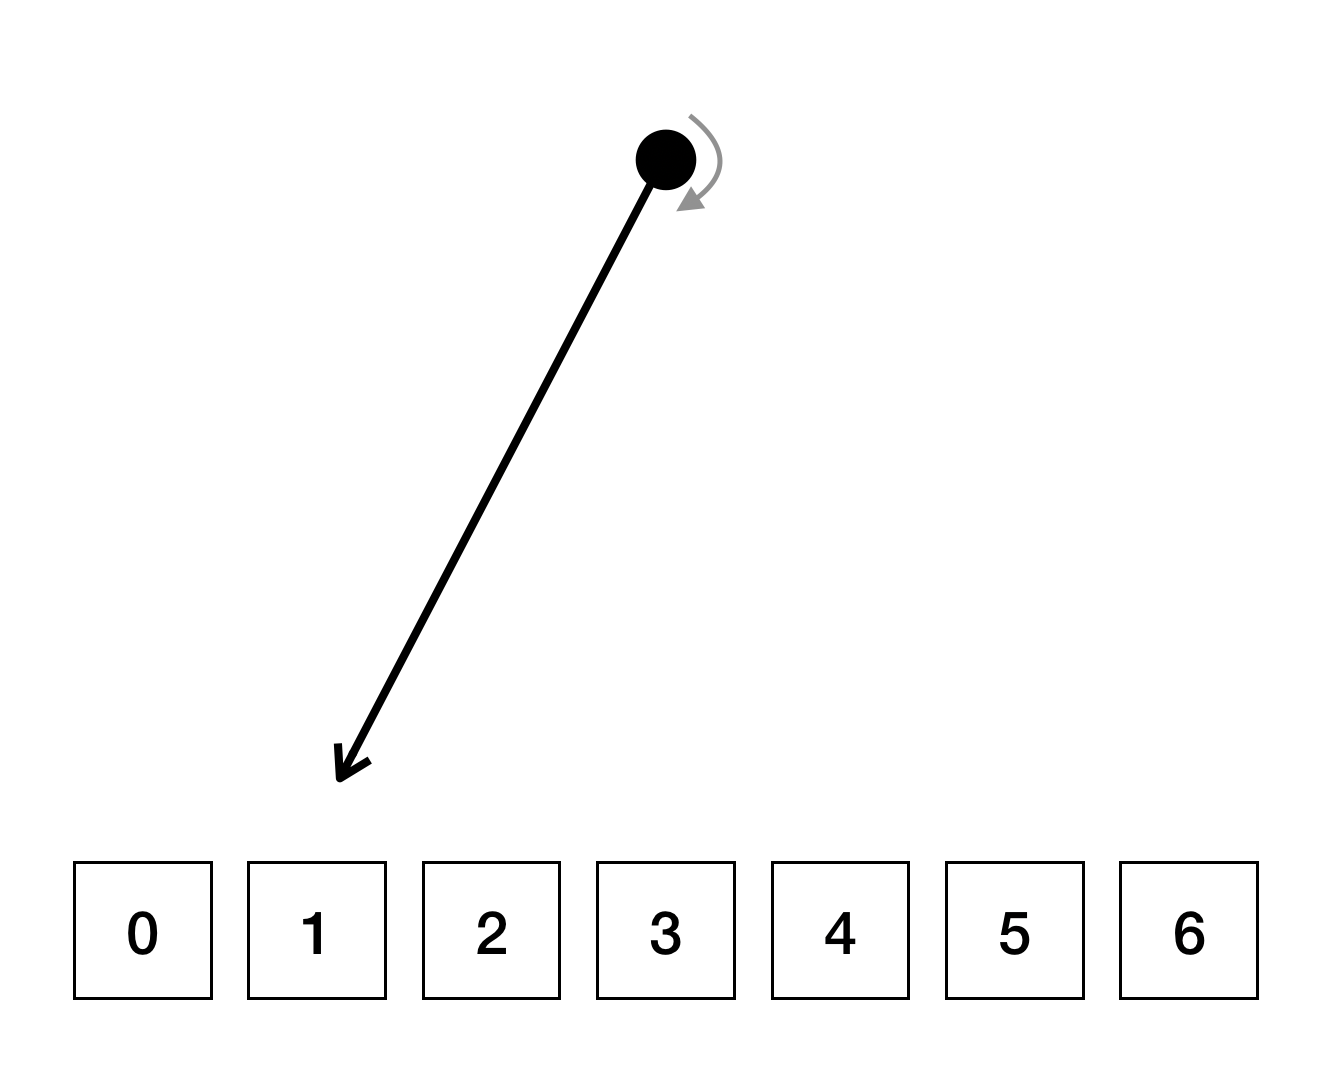
\includegraphics[width=0.7\textwidth]{pic5.png}
    \caption{“淘汰摆”当前指向Index为1的Cache块并处于向左摆动的过程中}
\end{figure}
如果新装入的Cache块属于偶尔使用1次就不再使用的块,“淘汰摆”在摆动到左端点后会继续向右摆动,从而能够很快的替换掉这一个Cache块。

如果新装入的Cache块属于接下来会很频繁使用的块,“淘汰摆”在装入这一个Cache块后,虽然有可能在后续的向右摆动中替换掉这一块,但是因为这个Cache块会频繁使用,因此会很快在被装入,当再次装入这一块时,“淘汰摆”会继续向右摆动,摆动到右端点才会回来,这会让这一个Cache块保留很长时间。


\subsection{实际测试与结果分析}





\section{实验总结}
本次实验中,我深入学习了主流替换策略的核心算法,并在模拟器上实现了自己的替换策略。实验证明,该策略相比LRU来说缺失率相近,相比随机算法来说缺失率降低,在某些数据上表现比较好。通过本次实验,我对Cache的工作方式理解更加深刻了。
\end{document}